\documentclass[11pt,a4paper]{article}
\usepackage[T1]{fontenc}
\usepackage{lmodern,amsmath,amssymb,booktabs,microtype,graphicx}
\usepackage[margin=24mm]{geometry}
\usepackage[colorlinks=true,urlcolor=blue,linkcolor=blue]{hyperref}
\newcommand{\dd}{\mathrm d}
\newcommand{\Js}{\mathcal J_s}
\newcommand{\Tr}{\operatorname{Tr}}
\DeclareMathOperator{\sech}{sech}
\title{From the derivative singlet to Rindler wavepackets\\A two-point construction and its four-point contour}
\author{Alan Day \and Chengheng\thanks{AI research assistant (OpenAI).}}
\date{Local research note --- 6 November 2026}
\begin{document}\maketitle
\begin{abstract}
We construct spatially smeared massive fields whose Rindler midpoint
correlator approaches the small-deformation derivative-singlet kernel.
The construction uses the established Kontorovich--Lebedev transform and
works for every positive mass. A Gaussian frequency regulator gives a
uniform two-point error bound and an exact radial norm. The resulting
free-field four-point function fixes what an ordinary thermal contour
would predict. It differs from the microscopic tracial fourth moment,
making the insertion contour, rather than a fit of decay rates, the next
dictionary problem. The bra/ket-dependent fake-circle map of Lin and
Stanford supplies the relevant existing framework.
\end{abstract}

\section{The microscopic input and a boost normalization}
Our starting observable is the conserved-subtracted derivative singlet
of complex DSSYK, in the full annealed normalized trace at $\beta=\mu=0$.
With standard CAR and the Hamiltonian normalization of the preceding
singlet notes, it is
\begin{align}
 X&=(O-cB)/\sqrt{W_d},\qquad O=\sum_i[H,c_i]^\dagger[H,c_i]-\mathbb E A(Q),\notag\\
 B&=H^2-\mathbb E H^2(Q),\quad c=2\lambda\frac{1-q}{1+q},\quad
 W_d=4\Js^4\left(\lambda^{-1}+\frac{4q}{1+q}\right),\qquad q=e^{-4\lambda}.
\end{align}
Here $A$ denotes the displayed sum before subtraction, and $Q$ is fermion
number. First take $N,p\to\infty$ at $p^2/N=\lambda>0$, then take
$\lambda\to0$ at fixed string time $t$. The established two-point result is
\begin{equation}
 \tau(X(t)X)\longrightarrow\sech^4(2\Js t),\qquad
 \tau(X^4)=2+q^4\longrightarrow3.\label{micro}
\end{equation}
All statements below use $\hbar=c_{\rm light}=1$. The bulk comparison is
a free scalar in flat $(1+1)$-dimensional Rindler space,
\begin{equation}
 ds^2=-\rho^2\dd\eta^2+\dd\rho^2,\qquad \rho>0,\qquad \beta_\eta=2\pi.
\end{equation}
The state is the Minkowski vacuum restricted to the right wedge. It is
thermal for boosts, with local proper temperature $1/(2\pi\rho)$
\cite{unruh,mssbulk}. This is the flat-space setting proposed for the
meson sector by Miyashita, Sekino and Susskind \cite{mssbulk}.

Set, as a candidate comparison of clocks,
\begin{equation}
 \eta=4\Js t,\qquad C(\eta)=\sech^4(\eta/2).\label{clock}
\end{equation}
This also makes the previously obtained string growth $e^{4\Js t}$
equal to boost growth $e^\eta$. It corresponds to inverse temperature
$\beta_t=\pi/(2\Js)$ for the comparison kernel. Rahman--Susskind's cord
formula has argument $\mathcal J_0 t_s$ and temperature
$\mathcal J_0/\pi$ \cite{rs}; matching arguments here sets
$\mathcal J_0=2\Js$. This is a normalization of the two kernels,
not a derivation of a particular observer radius. Proper time at fixed
$\rho_0$ would be $\tau_{\rm prop}=\rho_0\eta$.

\section{Thermal completion of the singlet spectrum}
Use the Fourier convention
\begin{equation}
 C(\eta)=\int_{\mathbb R}\frac{\dd\nu}{2\pi}
 S_C(\nu)e^{-i\nu\eta},\qquad
 S_C(\nu)=\frac{8\pi}{3}\frac{\nu(1+\nu^2)}{\sinh\pi\nu}.\label{spectrum}
\end{equation}
For example, substituting $y=e^\eta$ in the Fourier integral gives
$16B(2+i\nu,2-i\nu)=\frac83|\Gamma(2+i\nu)|^2$, which is
\eqref{spectrum}. In particular $S_C(0)=8/3$ and
$\int_0^\infty \nu^2S_C(\nu)\dd\nu/\pi=1$.

The even spectrum has a direct interpretation as a thermal midpoint,
or reflected left--right, correlator. If $W$ is the right-wedge
Wightman function, the relation and its spectral completion are
\begin{align}
 C(\eta)&=W(\eta-i\pi),&
 S_W(\nu)&=e^{\pi\nu}S_C(\nu),\label{midpoint}\\
 S_W(-\nu)&=e^{-2\pi\nu}S_W(\nu),&
 S_W(\nu)-S_W(-\nu)&=\frac{16\pi}{3}\nu(1+\nu^2).
\end{align}
The unregulated $W$ is a distribution; its positive-frequency spectrum
grows cubically. The midpoint is an ordinary analytic function in
$|\operatorname{Im}\eta|<\pi$. A trace gives an even same-operator
spectrum, whereas a finite-temperature Wightman function obeys detailed
balance. Thus \eqref{midpoint} specifies which correlator is being matched.
Evenness alone does not select a temperature: other spectral thermal
tilts are possible. Equation \eqref{clock} selects the Rindler comparison
with its conventional boost period.

\section{A spatial construction for every positive mass}
The standard massive Rindler modes \cite{unruh}, specialized to two
dimensions and normalized by the Klein--Gordon inner product, are
\begin{equation}
 u_\nu(\eta,\rho)=\frac{\sqrt{\sinh\pi\nu}}{\pi}
 K_{i\nu}(m\rho)e^{-i\nu\eta},\qquad \nu>0.\label{modes}
\end{equation}
Indeed the KL orthogonality relation has coefficient
$\pi^2/(2\nu\sinh\pi\nu)$, while the KG product contributes $2\nu$.
Expand $\phi=\int_0^\infty\dd\nu(a_\nu u_\nu+a_\nu^\dagger u_\nu^*)$
with $[a_\nu,a_{\nu'}^\dagger]=\delta(\nu-\nu')$.
For a real radial profile define
\begin{equation}
 \Phi_f(\eta)=\int_0^\infty\frac{\dd\rho}{\rho}f(\rho)\phi(\eta,\rho),
 \qquad F_f(\nu)=\int_0^\infty\frac{\dd\rho}{\rho}f(\rho)K_{i\nu}(m\rho).
\end{equation}
The Bose factors $n_\nu=(e^{2\pi\nu}-1)^{-1}$ give
\begin{align}
 W_f(\eta)&=\int_0^\infty\frac{\dd\nu}{\pi^2}\sinh(\pi\nu)|F_f(\nu)|^2
 \{(n_\nu+1)e^{-i\nu\eta}+n_\nu e^{i\nu\eta}\},\notag\\
 C_f(\eta)&=W_f(\eta-i\pi)
 =\frac1{\pi^2}\int_0^\infty\dd\nu\,|F_f(\nu)|^2\cos(\nu\eta).\label{cf}
\end{align}
The thermal factors have cancelled in the midpoint. We can therefore
construct a profile from a prescribed positive spectrum.

Choose a frequency resolution $\epsilon>0$ and set
\begin{align}
 F_\epsilon(\nu)&=\sqrt{\pi S_C(\nu)}\,e^{-\epsilon\nu^2/2},\label{fe}\\
 f_{m,\epsilon}(\rho)&=\frac2{\pi^2}\int_0^\infty\dd\nu\,
 \nu\sinh(\pi\nu)F_\epsilon(\nu)K_{i\nu}(m\rho).\label{inverse}
\end{align}
Equation \eqref{inverse} is the existing KL inverse, not a new transform
\cite{dlmf,yak}. Its $L^2$ formulation applies: in Yakubovich's
notation take the forward input to be $f_{m,\epsilon}(x/m)/x$.
Then \eqref{cf} becomes exactly
\begin{equation}
 C_\epsilon(\eta)=\int_0^\infty\frac{\dd\nu}{\pi}
 S_C(\nu)e^{-\epsilon\nu^2}\cos(\nu\eta)
 =e^{\epsilon\partial_\eta^2}C(\eta).\label{heat}
\end{equation}
For all real $\eta$, not just a finite plotting interval,
\begin{equation}
 |C_\epsilon(\eta)-C(\eta)|\leq
 \epsilon\int_0^\infty\frac{\dd\nu}{\pi}\nu^2S_C(\nu)=\epsilon.\label{bound}
\end{equation}
This follows from $0\leq1-e^{-x}\leq x$. For $\epsilon<1$,
normalizing $C_\epsilon(0)$ to one changes the bound to
$2\epsilon/(1-\epsilon)$. Here $\epsilon$ is a resolution parameter,
independent of the microscopic deformation $\lambda$.

KL Plancherel gives an exact measure of the spatial smearing:
\begin{align}
 \|f_{m,\epsilon}\|_{L^2(\dd\rho/\rho)}^2
 &=\frac2{\pi^2}\int_0^\infty\dd\nu\,\nu\sinh(\pi\nu)|F_\epsilon(\nu)|^2\notag\\
 &=\frac{16}{3}\int_0^\infty\dd\nu\,(\nu^2+\nu^4)e^{-\epsilon\nu^2}
 =\frac{4\sqrt\pi}{3\epsilon^{3/2}}+\frac{2\sqrt\pi}{\epsilon^{5/2}}.\label{norm}
\end{align}
For each positive $\epsilon$ the ordinary Wightman variance is also
finite: its integrand is proportional to
$S_C(\nu)e^{-\epsilon\nu^2}\cosh\pi\nu$.
These are well-defined smeared fields on the usual free-field domain.
Removing the regulator preserves the midpoint function but makes the
radial norm diverge. The exact unregulated kernel is not represented
by an $L^2(\dd\rho/\rho)$ profile of this form.

\begin{figure}[t]
\centering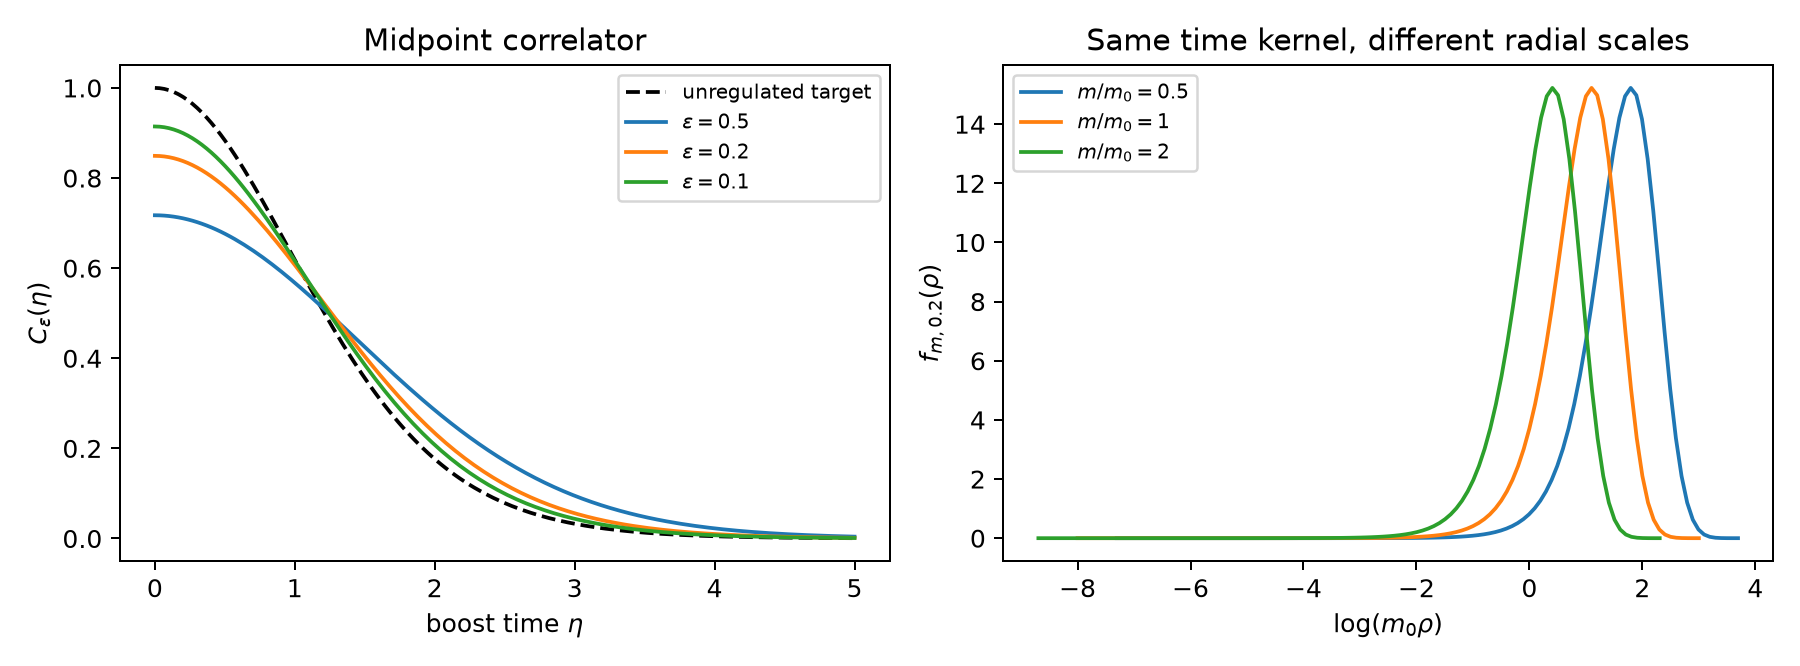
\includegraphics[width=\textwidth]{../../results/susskind-rindler-packet/rindler-packet.png}
\caption{Left: three regulated midpoint functions approaching the singlet
kernel. Right: at $\epsilon=0.2$, masses $m/m_0=0.5,1,2$ produce different
radial profiles but exactly the same temporal kernel. Profiles are
smearing functions, not particle probability densities.}
\end{figure}

The mass freedom is explicit. With a reference mass $m_0$,
\begin{equation}
 f_{m,\epsilon}(\rho)=f_{m_0,\epsilon}\bigl((m/m_0)\rho\bigr).\label{dilate}
\end{equation}
The measure $\dd\rho/\rho$ is invariant under this dilation. Consequently
neither the time kernel nor \eqref{norm} fixes $m$. This is a concrete
family of free-field realizations of our one-observable data, not a
candidate meson mass spectrum. A physical stretched-horizon location,
a locality constraint on $f$, or additional spatially resolved
observables can restrict this freedom.

\section{What the same bulk field predicts at four points}
Having constructed a field, its ordinary thermal four-point contour is
no longer adjustable independently. Write the equally spaced thermal
correlator schematically as
\begin{equation}
 F^{\rm eq}_\epsilon(\eta)=
 \langle\Phi_f(\eta)\Phi_f(0)\Phi_f(\eta)\Phi_f(0)\rangle_{\beta/4\ \mathrm{gaps}}.
\end{equation}
This denotes the analytic KMS contour with four imaginary-time gaps
$\beta/4=\pi/2$; it does not posit a trace-class density operator for an
infinite continuum wedge. Wick's theorem gives the exact free answer
\begin{equation}
 F^{\rm eq}_\epsilon(\eta)=C_\epsilon(0)^2+
 2\operatorname{Re}\{C_\epsilon(\eta+i\pi/2)^2\}.\label{four}
\end{equation}
The opposite pairs are separated by $\beta/2$; the adjacent pairs by
$\beta/4$ and $3\beta/4$, producing the two complex-conjugate terms.
As $\epsilon\downarrow0$, the shifted arguments remain inside the
midpoint strip. At zero real time,
\begin{equation}
 C(0)=1,\quad C(i\pi/2)=4,\qquad
 \lim_{\epsilon\downarrow0}F^{\rm eq}_\epsilon(0)=33.\label{33}
\end{equation}
This does not equal the microscopic limit $\tau(X^4)=3$ in
\eqref{micro}. Rescaling the bulk field to keep its midpoint variance
one does not remove the discrepancy. The specific rule ``match the
two-point midpoint, then identify ordinary equally spaced thermal
products'' therefore fails already at leading order. This calculation
does not test all possible multi-insertion dictionaries.

There is a useful existing route forward. Lin--Stanford's map
\cite{ls} is different for a bra and a ket insertion:
\begin{equation}
 \phi_{\rm ket}+\pi/2=v(\theta_{\rm ket}+\pi/2),\qquad
 \phi_{\rm bra}-\pi/2=v(\theta_{\rm bra}-\pi/2).\label{fake}
\end{equation}
Their small-deformation two-point inner product is proportional to
$\sin^{-2\Delta}[(\phi_{\rm bra}-\phi_{\rm ket})/2]$.
At $v\to0$, the two real arcs approach opposite points of the fake
circle, rather than a uniformly rescaled physical circle. Lorentzian
continuation must retain $v/\beta_B$ before sending $\beta_B\to0$.
This supports a midpoint comparison and directs us to their
multi-particle inner products, timefolds and two-sided OPE for the
four-point map. Their \S4.3 already gives a leading double-commutator
formula; it should be specialized with the actual insertion ordering.

Maldacena--Shenker--Stanford's Rindler example likewise distinguishes
the $\beta/4$-shifted four-point function and its Minkowski ordering
\cite{chaos}. A scattering interpretation needs those preparation
data as well as a growth exponent. In particular our known scrambling
function has the representation
\begin{equation}
 \mathcal F(z)=\mathbb E_{P,Q\sim\Gamma(4,1)}e^{-zPQ},\qquad
 z=(\lambda/2)e^\eta.
\end{equation}
A unitary phase $e^{iaPQ}$ corresponds to a continuation $z=-ia$,
not positive real $z$. The contour and external states must establish
that continuation before an on-shell coupling can be assigned.

\section{The next calculation}
The current construction supplies explicit candidate spatial smears
and a checkable thermal contour baseline. We will next specialize the
Lin--Stanford/Streicher multi-point formulas to the $r=q^2$ singlet,
retaining its same-species contractions, and compare their
$O(\lambda)$ double commutator to the existing exact chord OTOC.
This can fix the insertion prescription without guessing it from
the two-point function. The string-clock short-time coefficient
$1280\Js^2\lambda t^2$ and the late overlap
$16\lambda e^{4\Js t}$ provide two separate checks.

Mass extraction then requires an independently defined radial or
translation observable and a cross-correlator matrix for more than
one singlet. The present mass-dilation family explains precisely why
one temporal spectrum is insufficient. The conformal chord label
$\Delta=2$ alone is not a $(1+1)$-dimensional Poincare mass. Finite
curvature and interacting meson scattering remain subsequent steps.

\appendix
\section{A finite-algebra check of thermal dressing}
For any finite Hermitian $H$, let $\tau=\Tr/d$,
$Z_\beta=\tau(e^{-\beta H})$ and
$\rho_\beta=e^{-\beta H}/Z_\beta$ (a density relative to $\tau$).
The fixed dressing
\begin{equation}
 A_2=\sqrt{Z_\beta}\,e^{\beta H/4}Xe^{\beta H/4}
\end{equation}
satisfies the exact identity
$\tau(\rho_\beta^{1/2}A_2(t)\rho_\beta^{1/2}A_2)=\tau(X(t)X)$.
At four points the same dressing instead gives
\begin{equation}
 \tau\!\left[\prod_{j=1}^4\rho_\beta^{1/4}A_2(t_j)\right]
 =Z_\beta\tau\!\left[\prod_{j=1}^4X(t_j)e^{\beta H/4}\right].
\end{equation}
To cancel $n$ equal thermal gaps in this manner requires
$A_n=Z_\beta^{1/n}e^{\beta H/(2n)}Xe^{\beta H/(2n)}$.
Its dependence on $n$ is why this construction is a two-point
reweighting, not a single product-preserving operator map. The
continuum Rindler construction in the main text uses KMS functions,
not an assumption that this finite density matrix exists there.

\section{Numerical record and reproducibility}
\begin{center}
\begin{tabular}{rrrr}
\toprule
$\epsilon$ & $C_\epsilon(0)$ & $\|f\|^2$ & $F^{\rm eq}_\epsilon(0)/C_\epsilon(0)^2$\\
\midrule
0.50 & 0.717380 & 26.7374 & 7.49122\\
0.20 & 0.849207 & 224.589 & 12.3802\\
0.10 & 0.914388 & 1195.73 & 17.4203\\
0.05 & 0.953942 & 6552.70 & 22.5386\\
0.01 & 0.990171 & 356854 & 30.1092\\
\bottomrule
\end{tabular}
\end{center}
The main run performs 91 checks: Fourier integrals, heat versus
spectral convolution, spectral norm, the uniform regulator bound,
finite-matrix dressings, and 21 radial refinements. Radial profiles
use 128 Gauss--Legendre nodes on $[0,32]$, 25-digit Bessel evaluations,
and float64 final sums; selected comparisons use 256 nodes on $[0,40]$
and 40-digit Bessel evaluations. Their largest absolute difference
is $6.6\times10^{-13}$. Near $\log(m\rho)=-8$ the cancellation condition
reaches $4.9\times10^8$, so absolute agreement does not imply the same
relative precision there.

An independent script uses 50-digit tanh--sinh integration at four
radial points, finite-oscillator thermal traces for \eqref{four},
and spatial Simpson norms on the plotted box. Numerical refinements
give radial absolute differences below $5.7\times10^{-13}$, with relative
error $1.1\times10^{-6}$ at the smallest-amplitude point. The nine oscillator
comparisons differ by at most $8.9\times10^{-16}$; the largest finite-box
norm discrepancy is $4.1\times10^{-10}$ relative. These refinements
are empirical; no interval bound on radial quadrature or the omitted
spatial tail is claimed. Equations \eqref{bound} and \eqref{norm} are
analytic statements about the full integrals.

Code is in \texttt{code/rindler\_singlet\_packet.py} and the corresponding
\texttt{run\_} and \texttt{check\_} scripts. The result directory is
\path{results/susskind-rindler-packet/}. It records data, parameters,
dependency versions and input hashes. The build script runs
\texttt{pdflatex} twice; the local manifest binds source, output and
rendered-page hashes. This stage is saved locally without a Git commit
or push.

\begin{thebibliography}{9}
\small\setlength{\itemsep}{3pt}
\bibitem{mssbulk} S.~Miyashita, Y.~Sekino and L.~Susskind,
\emph{DSSYK at Infinite Temperature: The Flat-Space Limit and the 't Hooft Model},
\href{https://arxiv.org/abs/2506.18054}{arXiv:2506.18054v3}, \S\S5.3,6.
\bibitem{rs} A.~Rahman and L.~Susskind,
\emph{Infinite Temperature is Not So Infinite: The Many Temperatures of de Sitter Space},
\href{https://arxiv.org/abs/2401.08555}{arXiv:2401.08555v3}, (4.42)--(5.47).
\bibitem{unruh} L.~C.~B.~Crispino, A.~Higuchi and G.~E.~A.~Matsas,
\emph{The Unruh effect and its applications},
\href{https://arxiv.org/abs/0710.5373}{arXiv:0710.5373},
\S\S II.C--II.E and Appendix A; PDF (2.92).
\bibitem{dlmf} NIST Digital Library of Mathematical Functions,
\href{https://dlmf.nist.gov/10.43.v}{\S10.43(v)}, (10.43.30)--(10.43.31).
\bibitem{yak} S.~B.~Yakubovich,
\emph{Uncertainty principles for the Kontorovich--Lebedev transform},
Math. Model. Anal. \textbf{13} (2008) 289--302,
\href{https://doi.org/10.3846/1392-6292.2008.13.289-302}{doi:10.3846/1392-6292.2008.13.289-302},
(1.1)--(1.3), (4.1).
\bibitem{ls} H.~W.~Lin and D.~Stanford,
\emph{A symmetry algebra in double-scaled SYK},
\href{https://arxiv.org/abs/2307.15725}{arXiv:2307.15725},
\S\S4.2--4.6, (158)--(159), (167), (170), (181).
\bibitem{chaos} J.~Maldacena, S.~H.~Shenker and D.~Stanford,
\emph{A bound on chaos},
\href{https://arxiv.org/abs/1503.01409}{arXiv:1503.01409}, Appendix A.
\end{thebibliography}
\end{document}
